% !TEX TS-program = pdflatexmk
\RequirePackage{iftex}
\ifPDFTeX
  \pdfoutput=1
  \pdfminorversion=7
  \input glyphtounicode
  \pdfgentounicode=1
\fi
\ifdefined\pdfinterwordspaceon\pdfinterwordspaceon\fi
\documentclass[justified,notoc,twoside,nobib,nofonts]{tufte-handout}
\usepackage[T1]{fontenc}
\usepackage[utf8]{inputenc}
\usepackage[english]{babel}
\ifPDFTeX
  \usepackage[tracking]{microtype}
\else
  \usepackage{microtype}
\fi
\usepackage{amsthm,thmtools,thm-restate}
\usepackage{amsmath,amssymb,mathtools}
% KPfonts text, with the same New PX maths as the font comparison.
\usepackage[nomath,oldstylenums]{kpfonts}
\edef\KPbodyfamily{\rmdefault}
\renewcommand{\rmdefault}{zpltlf}
\usepackage{newpxmath}
\let\rmdefault\KPbodyfamily
\renewcommand{\familydefault}{\rmdefault}

% BaskervilleF headings use native Type 1 fonts and work with pdfLaTeX.
\newcommand{\BaskervilleHeading}{%
  \fontencoding{T1}\fontfamily{BaskervilleF-LF}%
  \fontseries{m}\fontshape{n}\selectfont}
\titleformat{\section}[hang]
  {\BaskervilleHeading\fontsize{15}{18}\selectfont}
  {\thesection}{1em}{}
\titleformat{\subsection}[hang]
  {\BaskervilleHeading\fontsize{13}{16}\selectfont}
  {\thesubsection}{1em}{}
\titleformat{\paragraph}[runin]
  {\BaskervilleHeading}{\theparagraph}{1em}{}
\usepackage{etoolbox}
\makeatletter
\patchcmd{\maketitle}{\LARGE\itshape\@title}
  {\BaskervilleHeading\fontsize{22}{26}\selectfont\@title}
  {}{\PackageError{strong-five-cdc}{Title font patch failed}{}}
% The author and email are printed immediately below the title block.
\patchcmd{\maketitle}{\@@author\@@date}{\@@date}
  {}{\PackageError{strong-five-cdc}{Author block patch failed}{}}
\makeatother
\usepackage{booktabs,array,enumitem,needspace}
\usepackage[numbers,square]{natbib}
\usepackage{tikz}
\usetikzlibrary{arrows.meta}
\usepackage{xurl,hyperref,cleveref}
\usepackage{accsupp}
\urlstyle{same}
\geometry{a4paper,top=23mm,bottom=46mm,left=28mm,right=56mm,marginparwidth=3cm}
\setlength{\emergencystretch}{2em}
\clubpenalty=10000
\widowpenalty=10000
\displaywidowpenalty=10000
\setcounter{secnumdepth}{2}
\AtBeginDocument{\fontsize{12}{15}\selectfont}
\fancyhead[LE]{\thepage\quad\textsmallcaps{nikolay ulyanov}}
\fancyhead[RO]{\textsmallcaps{gp III.2}\quad\thepage}
\declaretheorem[name=Theorem,numberwithin=section]{theorem}
\declaretheorem[name=Proposition,sibling=theorem]{proposition}
\declaretheorem[name=Lemma,sibling=theorem]{lemma}
\declaretheorem[name=Corollary,sibling=theorem]{corollary}
\declaretheorem[name=Definition,sibling=theorem,style=definition]{definition}
\setlist[enumerate]{label=\textup{(\roman*)},leftmargin=*,itemsep=2pt,topsep=4pt}
\newcommand{\F}{\mathbb F_2}
\newcommand{\K}{\mathbb F_2^2}
\newcommand{\sd}{\mathbin{\triangle}}
\newcommand{\supp}{\operatorname{supp}}
\newcommand{\df}{\operatorname{df}}
\newcommand{\pair}[2]{\left\langle #1,#2\right\rangle}
\newcommand{\word}[1]{\texttt{#1}}
\setcitestyle{numbers,square}

% Full references appear in the margin at their first citation.
% Use the selection fix from snark_book_opus/book/preamble.tex:
% margin notes stay visible but do not enter the main copied text.
\makeatletter
\newdimen\@gp@fnmarkwidth
\newcommand{\bothcite}[2][0cm]{%
  \citep{#2}\sidenote[][#1]{\raggedright\csname paper@#2\endcsname}%
  \kern\@gp@fnmarkwidth\@gp@cite@space}
\def\@gp@cite@space{\@ifnextchar.{\@gp@cite@halfspace}{\@gp@cite@comma}}
\def\@gp@cite@comma{\@ifnextchar,{\@gp@cite@halfspace}{\@gp@cite@semicolon}}
\def\@gp@cite@semicolon{\@ifnextchar;{\@gp@cite@halfspace}{\@gp@cite@colon}}
\def\@gp@cite@colon{\@ifnextchar:{\@gp@cite@halfspace}{\@gp@cite@exclamation}}
\def\@gp@cite@exclamation{\@ifnextchar!{\@gp@cite@halfspace}{\@gp@cite@question}}
\def\@gp@cite@question{\@ifnextchar?{\@gp@cite@halfspace}{\@gp@cite@openparen}}
\def\@gp@cite@openparen{\@ifnextchar({\@gp@cite@halfspace}{\@gp@cite@closeparen}}
\def\@gp@cite@closeparen{\@ifnextchar){\@gp@cite@halfspace}{\@gp@cite@bracket}}
\def\@gp@cite@bracket{\@ifnextchar]{\@gp@cite@halfspace}{\@gp@cite@normalspace}}
\def\@gp@cite@halfspace{\nobreak\hskip.5\fontdimen2\font\relax}
\def\@gp@cite@normalspace{\nobreak\space}
\ifPDFTeX
\def\@makefnmark{%
  \hbox{%
    \setbox\z@=\hbox{\@textsuperscript{\normalfont\footnotesize\@thefnmark}}%
    \global\@gp@fnmarkwidth=\wd\z@%
    \setbox\tw@=\copy\z@%
    \immediate\pdfxform\tw@%
    \pdfannot width\wd\z@ height\ht\z@ depth\dp\z@{%
      /Subtype /Watermark /F 708 /Contents ()%
      /AP << /N \the\pdflastxform\space 0 R >>%
    }%
  }%
}
\fi
\renewcommand\@footnotetext[2][0pt]{%
  \marginpar{%
    \BeginAccSupp{method=hex,unicode,ActualText=2060}%
    \hbox{}\vspace*{#1}%
    \def\baselinestretch{\setspace@singlespace}%
    \reset@font\footnotesize%
    \@tufte@margin@par%
    \vspace*{-1\baselineskip}\noindent%
    \protected@edef\@currentlabel{%
      \csname p@footnote\endcsname\@thefnmark%
    }%
    \color@begingroup%
      \@makefntext{\ignorespaces#2}%
    \color@endgroup%
    \EndAccSupp{}%
  }%
}
\renewcommand\marginnote[2][0pt]{%
  \ifthenelse{\boolean{@tufte@loadnatbib}}{%
    \let\cite\@tufte@infootnote@cite%
  }{}%
  \gdef\@tufte@citations{}%
  \marginpar{%
    \BeginAccSupp{method=hex,unicode,ActualText=2060}%
    \hbox{}\vspace*{#1}%
    \@tufte@marginnote@font\@tufte@marginnote@justification%
    \@tufte@margin@par\vspace*{-1\baselineskip}\noindent #2%
    \EndAccSupp{}%
  }%
  \@tufte@print@citations%
  \ifthenelse{\boolean{@tufte@loadnatbib}}{%
    \let\cite\@tufte@normal@cite%
  }{}%
}
\expandafter\def\csname paper@HO13\endcsname{%
  Arthur Hoffmann-Ostenhof. \emph{A note on 5-cycle double covers}.
  Graphs and Combinatorics 29(4) (2013), 977--979.
  \href{https://doi.org/10.1007/s00373-012-1169-8}{\nolinkurl{doi:10.1007/s00373-012-1169-8}}.}
\expandafter\def\csname paper@HOZZ19\endcsname{%
  Arthur Hoffmann-Ostenhof, Cun-Quan Zhang and Zhang Zhang.
  \emph{Cycle double covers and non-separating cycles}.
  European Journal of Combinatorics 81 (2019), 276--284.
  \href{https://doi.org/10.1016/j.ejc.2019.06.006}{\nolinkurl{doi:10.1016/j.ejc.2019.06.006}}.}
\expandafter\def\csname paper@HS26\endcsname{%
  Radek Hu\v{s}ek and Robert \v{S}\'amal.
  \emph{Exponentially many circuit double covers}.
  2026. \href{https://arxiv.org/abs/2607.24724}{arXiv:2607.24724}.}
\expandafter\def\csname paper@LHLZ23\endcsname{%
  Siyan Liu, Rong-Xia Hao, Rong Luo and Cun-Quan Zhang.
  \emph{5-cycle double covers, 4-flows, and Catlin reduction}.
  SIAM Journal on Discrete Mathematics 37(1) (2023), 253--267.
  \href{https://doi.org/10.1137/22M1472425}{\nolinkurl{doi:10.1137/22M1472425}}.}
\expandafter\def\csname paper@LHLZ25\endcsname{%
  Xiaoyu Li, Rong-Xia Hao, Rong Luo and Cun-Quan Zhang.
  \emph{Non-separating cycles and 5-cycle double covers}.
  Discrete Mathematics 348(9) (2025), 114515.
  \href{https://doi.org/10.1016/j.disc.2025.114515}{\nolinkurl{doi:10.1016/j.disc.2025.114515}}.}
\expandafter\def\csname paper@Xu14\endcsname{%
  Rui Xu. \emph{Strong 5-cycle double covers of graphs}.
  Graphs and Combinatorics 30(2) (2014), 495--499.
  \href{https://doi.org/10.1007/s00373-012-1266-8}{doi:10.1007/s00373-012-1266-8}.}
\expandafter\def\csname paper@U26\endcsname{%
  Nikolay Ulyanov. \emph{Graph Puzzles III.1: A proof of Sabidussi's
  compatibility conjecture with 4 colours}.
  2026.
  \href{https://arxiv.org/abs/2607.13225}{arXiv:2607.13225}.}
\expandafter\def\csname paper@KMNS24\endcsname{%
  J\'an Karab\'a\v{s}, Edita M\'a\v{c}ajov\'a, Roman Nedela and
  Martin \v{S}koviera. \emph{Cubic graphs with colouring defect 3}.
  Electronic Journal of Combinatorics 31(2) (2024), P2.6.
  \href{https://doi.org/10.37236/12333}{doi:10.37236/12333}.}
\expandafter\def\csname paper@MS21\endcsname{%
  Edita M\'a\v{c}ajov\'a and Martin \v{S}koviera.
  \emph{Critical and flow-critical snarks coincide}.
  Discussiones Mathematicae Graph Theory 41(2) (2021), 503--511.
  \href{https://doi.org/10.7151/dmgt.2204}{\nolinkurl{doi:10.7151/dmgt.2204}}.}
\expandafter\def\csname paper@MS25\endcsname{%
  Edita M\'a\v{c}ajov\'a and Martin \v{S}koviera.
  \emph{Are there any permutation snarks on $6\pmod 8$ vertices?}
  Procedia Computer Science 273 (2025), 163--168.
  \href{https://doi.org/10.1016/j.procs.2025.10.294}{\nolinkurl{doi:10.1016/j.procs.2025.10.294}}.}
\expandafter\def\csname paper@S01\endcsname{%
  Eckhard Steffen. \emph{On bicritical snarks}.
  Mathematica Slovaca 51(2) (2001), 141--150.
  \href{https://dml.cz/dmlcz/136800}{DML-CZ:136800}.}
\expandafter\def\csname paper@S15\endcsname{%
  Eckhard Steffen. \emph{1-factor and cycle covers of cubic graphs}.
  Journal of Graph Theory 78(3) (2015), 195--206.
  \href{https://doi.org/10.1002/jgt.21798}{\nolinkurl{doi:10.1002/jgt.21798}}.}
\newcommand{\paperreference}[1]{\csname paper@#1\endcsname}
\makeatother

\title[Graph Puzzles III.2-preview: Strong five-cycle double covers]{Graph Puzzles III.2-preview: Strong five-cycle double covers}
\author{Nikolay Ulyanov + AI-Slop}
\date{6 October 2026}
\hypersetup{pdftitle={Graph Puzzles III.2-preview: Strong five-cycle double covers},pdfauthor={Nikolay Ulyanov + AI-Slop},
  colorlinks=true,linkcolor=blue!50!black,citecolor=blue!50!black,urlcolor=blue!50!black}

\begin{document}
\selectlanguage{english}
\maketitle
Nikolay Ulyanov\textsuperscript{*} + AI-Slop%
\marginnote{\textsuperscript{*}{\scriptsize\href{mailto:ulyanick@gmail.com}{ulyanick@gmail.com}}}\par

\begin{abstract}
\noindent\newthought{Abstract: }
We prove that a circuit $C$ of a cubic graph $G$ is a member of a
five-cycle double cover whenever $G-V(C)$ is 3-edge-colourable.
The reverse implication is known.
The proof uses the bilinear balancing lemma from the proof of
Sabidussi's compatibility conjecture. It follows that every circuit
in a critical or permutation snark is a member of a five-cycle double
cover. We also prove the strong five-cycle double cover property
when $G$ has an induced hexagon $H$ and $G-E(H)$ has a proper
3-edge-colouring whose spoke colours, in cyclic order, are
$1,1,2,2,3,3$. The characterisation of snarks of colouring defect three
by such a hexagon gives this property for all these snarks.
\end{abstract}
\noindent\rule{\linewidth}{0.4pt}

\section{Introduction}\label{sec:introduction}

A \emph{circuit} is a nonempty connected 2-regular subgraph. A
\emph{cycle} is an even subgraph, identified with its edge set. A
\emph{$k$-cycle double cover} is an indexed family of at most $k$ cycles
in which every edge occurs twice. Empty members may be adjoined, and
repeated members retain their multiplicities. In a cubic graph, each
cycle is a union of vertex-disjoint circuits.

We say that a cubic graph has the \emph{strong $k$-cycle double cover
property} if every circuit is a component of a member of some
$k$-cycle double cover. We follow the convention of
Hoffmann-Ostenhof \bothcite{HO13}. Requiring the circuit itself to be a
member is stronger than requiring it to be a component of a member.

Throughout the paper graphs are finite and loopless, with
parallel edges allowed. The contraction $G/C$ retains the edges outside
$C$, including loops created by contraction. Our first result
characterises the circuits that are members of five-cycle double covers.

\begin{samepage}
\begin{restatable}[Prescribed circuit]{theorem}{prescribedcircuit}\label{thm:exact}
Let $G$ be a connected cubic graph and let $C$ be a circuit of $G$.
The following conditions are equivalent.
\begin{enumerate}
\item $G$ has a five-cycle double cover with $C$ as a member.
\item $G-V(C)$ has a proper 3-edge-colouring.
\item $G-E(C)$ has a proper 3-edge-colouring.
\item $G/C$ has a nowhere-zero $\K$-flow.
\end{enumerate}
\end{restatable}
\end{samepage}

\Needspace{4\baselineskip}
Li, Hao, Luo and Zhang \bothcite{LHLZ25}, Lemma~5.8, prove
(i)$\Rightarrow$(iv) for every cycle $C$, without assuming that
$G-E(C)$ is connected.
Hoffmann-Ostenhof, Zhang and Zhang \bothcite{HOZZ19},
Theorem~3.1, proved (iv)$\Rightarrow$(i) for a
non-separating cycle, meaning that $G-E(C)$ is connected.
Li et al. also treat non-separating cycles under bounds on the rank of
the cycle space of $G-E(C)$ and the number of components of $C$;
see \citep[Theorem~1.6]{LHLZ25}. We remove the connectedness assumption
in the sufficiency direction for circuits in cubic graphs.

The final step uses the construction from two even subgraphs in
Liu, Hao, Luo and Zhang \bothcite{LHLZ23}, Theorem~1.6.
To satisfy its hypotheses, we permute the three edge colours
independently in the components of $G-E(C)$. The parity lemma in
\cref{sec:balancing} chooses these permutations so that the resulting
flow on $G$ has an even number of endpoints of zero-valued edges in
each component of $G-E(C)$. A $T$-join then gives the second cycle
needed for the construction.

A cubic graph $G$ is \emph{critical} if $G-\{u,v\}$ is
3-edge-colourable for every edge $uv$. A \emph{cubic permutation graph}
has a spanning 2-factor $A\cup B$ consisting of two induced circuits.
Its remaining edges form a perfect matching between $A$ and $B$.
We use \emph{snark} for a connected bridgeless cubic graph of chromatic
index four. A \emph{critical snark} is a snark satisfying the first
condition; a \emph{permutation snark} is a snark satisfying the second.
The results also apply under the customary additional girth and
connectivity conditions.

\begin{restatable}[Critical and permutation graphs]{theorem}{criticalpermutation}\label{thm:classes}
Every connected critical cubic graph and every cubic permutation graph has a
five-cycle double cover with any prescribed circuit as a member.
In particular, critical snarks and permutation snarks have the strong
five-cycle double cover property.
\end{restatable}

The next theorem concerns a single induced hexagon and its six
incident edges. It will give the result for snarks of colouring defect
three.

\begin{restatable}[An induced hexagon]{theorem}{inducedhexagon}\label{thm:hexagon}
Let $G$ be a connected cubic graph with an induced hexagon
$H=v_0v_1\dots v_5v_0$. Suppose that $G-E(H)$ has a proper
3-edge-colouring in which the spokes at $v_0,\dots,v_5$ have colours
$1,1,2,2,3,3$, respectively. Then every circuit of $G$ is a component
of a member of a five-cycle double cover.
\end{restatable}

\Needspace{7\baselineskip}
The \emph{colouring defect} $\df(G)$ is the minimum number of edges
uncovered by a triple of perfect matchings. The characterisation of
Karab\'a\v{s}, M\'a\v{c}ajov\'a, Nedela and \v{S}koviera
\bothcite{KMNS24}, Theorem~3.3, supplies the hexagon and
edge-colouring required by \cref{thm:hexagon} when $\df(G)=3$.

\begin{restatable}{corollary}{defectthree}\label{cor:defect}
Every snark of colouring defect three has the strong five-cycle double
cover property.
\end{restatable}

\subsection{Formalization}
All of the results have also been formalized in Lean. The formalization is
available in the author's GitHub repository:
\href{https://github.com/gexahedron/graph-puzzles-lean}
{\nolinkurl{https://github.com/gexahedron/graph-puzzles-lean}}.

\subsection{Statement of AI use}
The proofs in this paper have been produced in a continuous dialog with AI, building upon the work done in \bothcite{U26} and some other unreleased work.


\section{A parity lemma for cyclic sequences}\label{sec:balancing}

For $x=(x_1,x_2)$ and $y=(y_1,y_2)$ in $\K$, put
\[
  \pair{x}{y}=x_1y_2+x_2y_1,\qquad q(x)=x_1x_2.
\]
The bilinear form is symmetric and alternating, and
\begin{equation}\label{eq:quadratic}
  q(x+y)=q(x)+q(y)+\pair{x}{y}.
\end{equation}
For an even-sized list of vectors in $\K$, each of the four vectors
occurs an even number of times exactly when the vector sum and the sum
of the $q$-values both vanish. Indeed, if $n_{rs}$ is the multiplicity
of $(r,s)$ modulo two, these two conditions give
$n_{10}=n_{11}$, $n_{01}=n_{11}$ and $n_{11}=0$; the parity of the
list length then gives $n_{00}=0$.

The bilinear balancing lemma in \citep{U26}, Lemma~5.1,
has the following consequence for a set of three choices.

\Needspace{12\baselineskip}
\begin{lemma}\label{lem:balancing}
Let $U$ be a finite set and let $\Sigma$ have three elements. For
distinct $u,v\in U$, suppose that
$\beta_{uv}:\Sigma\times\Sigma\to\F$ satisfies
\[
  \beta_{uv}(r,s)=\beta_{vu}(s,r),\qquad
  \sum_{s\in\Sigma}\beta_{uv}(r,s)=0.
\]
There are choices $t_u\in\Sigma$ such that
\[
  \sum_{v\ne u}\beta_{uv}(t_u,t_v)=0\qquad(u\in U).
\]
\end{lemma}

\begin{proof}
Identify $\Sigma$ with $\K\setminus\{0\}$. A function on these three
vectors whose values sum to zero extends uniquely to a linear map
$\K\to\F$: two of the vectors form a basis, and the third is their
sum. For each $\beta_{uv}$, the row sums vanish by hypothesis, and
the column sums vanish by transpose symmetry and the row-sum condition
for $\beta_{vu}$. Thus $\beta_{uv}$ extends uniquely to a bilinear map
$\K\times\K\to\F$, with transpose symmetry preserved.
The bilinear balancing lemma of \citep[Lemma~5.1]{U26}
provides nonzero vectors satisfying the displayed equations.
Restricting to $\Sigma$ gives the assertion.
\end{proof}

For a cyclic sequence $w_0,\dots,w_{n-1}$ of elements of $U$, put
$I_u=\{i:w_i=u\}$. Join consecutive positions by edges, with
indices read modulo $n$. We write $x_i$ for the colour of the edge
from position $i$ to position $i+1$; the two edge colours incident
with position $i$ are therefore $x_{i-1}$ and $x_i$.

\Needspace{18\baselineskip}
\begin{lemma}\label{lem:word}
Let $U$ be a finite set, let $\Sigma$ be a set of three elements,
and let $w_0,\dots,w_{n-1}$ be a cyclic sequence of elements of $U$.
For each $u\in U$ and $t\in\Sigma$,
let $\Delta_{u,t}:I_u\to\K\setminus\{0\}$
satisfy
\begin{equation}\label{eq:patterns}
  \sum_{i\in I_u}\Delta_{u,t}(i)=0,\qquad
  \sum_{t\in\Sigma}\Delta_{u,t}(i)=0.
\end{equation}
There are choices $t_u\in\Sigma$ and edge colours
$x_0,\dots,x_{n-1}\in\K$
such that
\[
  x_{i-1}+x_i=\Delta_{w_i,t_{w_i}}(i)
\]
and, for every $u$ and $z\in\K$, the number of incidences of colour
$z$ in $(x_{i-1},x_i)_{i\in I_u}$ is even.
\end{lemma}

\begin{proof}
Use the order $0<1<\dots<n-1$ to define, for $u\ne v$,
\[
 \beta_{uv}(t,s)=
 \sum_{\substack{i\in I_u,\ j\in I_v\\j<i}}
   \pair{\Delta_{u,t}(i)}{\Delta_{v,s}(j)}.
\]
Every pair in $I_u\times I_v$ occurs in one of the two orders. Hence
\[
 \beta_{uv}(t,s)+\beta_{vu}(s,t)
 =\pair{\sum_{i\in I_u}\Delta_{u,t}(i)}
        {\sum_{j\in I_v}\Delta_{v,s}(j)}=0.
\]
The second condition in \eqref{eq:patterns} also gives
$\sum_s\beta_{uv}(t,s)=0$. Choose $t_u$ by \cref{lem:balancing},
and write $y_i=\Delta_{w_i,t_{w_i}}(i)$. Set
\[
  x_{-1}=0,\qquad x_i=\sum_{j=0}^{i}y_j.
\]
The sum of all $y_i$ is zero, so $x_{n-1}=x_{-1}$ and the edge
colours are consistent around the cyclic sequence. Their successive
differences are the required nonzero vectors.

Fix $u$. The vector sum of the $2|I_u|$ incident edge colours is
$\sum_{i\in I_u}y_i=0$. By \eqref{eq:quadratic}, their quadratic sum is
\begin{align*}
 \sum_{i\in I_u}\bigl(q(x_{i-1})+q(x_i)\bigr)
 &=\sum_{i\in I_u}q(y_i)
   +\sum_{\substack{i\in I_u\\j<i}}\pair{y_i}{y_j}\\
 &=q\left(\sum_{i\in I_u}y_i\right)
   +\sum_{v\ne u}\beta_{uv}(t_u,t_v)=0.
\end{align*}
In the second equality, the terms with both indices in $I_u$ combine
with the individual $q$-values by repeated application of
\eqref{eq:quadratic}. The parity criterion at the start of this
section proves the assertion.
\end{proof}

The \emph{boundary} of an edge set is the set of its odd-degree
vertices. An edge set with boundary $T$ is called a \emph{$T$-join}.
We will use the following standard criterion.

\Needspace{8\baselineskip}
\begin{lemma}[$T$-joins]\label{lem:join}
Let $R$ be a graph and let $T$ be a set of its vertices. There is an
edge set $J\subseteq E(R)$ with boundary $T$ if and only if every
component of $R$ contains an even number of vertices of $T$.
\end{lemma}

\begin{proof}
The sum of degrees in a component is even, which proves necessity.
For sufficiency, pair the vertices of $T$ within each component, join
each pair by a path, and take the symmetric difference of the path
edge sets. Each internal vertex contributes even degree and the
resulting boundary is $T$.
\end{proof}

\section{A prescribed circuit as a member}\label{sec:exact}

A $\K$-flow assigns a vector to each edge so that the sum of the
incident values at each vertex is zero; a loop has two incidences.
A flow is \emph{nowhere zero} when every edge value belongs to
$\K\setminus\{0\}$.

\Needspace{14\baselineskip}
\prescribedcircuit*
\begin{proof}
We first prove the equivalence of (ii), (iii) and (iv).
A proper 3-edge-colouring of $G-E(C)$ restricts to $G-V(C)$.
Conversely, at each vertex outside $C$, assign its unused
colours to the edges joining it to $C$. In $G-E(C)$ every vertex of
$C$ has degree one. Assign any colour to each chord of $C$. This
extends a colouring of $G-V(C)$ to a proper colouring of $G-E(C)$.

Identify the three colours with the nonzero vectors of $\K$. A
proper colouring of $G-E(C)$ satisfies flow conservation at every
vertex outside $C$, since three distinct nonzero vectors sum to zero.
Summing over those vertices also gives conservation at the contracted
vertex of $G/C$. Conversely, a nowhere-zero $\K$-flow on $G/C$
has three distinct values at every cubic vertex outside $C$, and
therefore colours $G-E(C)$ properly. This proves the equivalence of
conditions (ii)--(iv).

Assume (iii), and let $f$ be the resulting nonzero edge values outside
$C$. Write $C=v_0e_0v_1e_1\dots v_{n-1}e_{n-1}v_0$, where
$e_i=v_iv_{i+1}$, and let $a_i$ be the unique edge outside $C$ at $v_i$.
For a component $B$ of $G-E(C)$, let $I_B=\{i:v_i\in V(B)\}$.
Summing conservation over the vertices of $B$ outside $C$ gives
\begin{equation}\label{eq:boundarysum}
  \sum_{i\in I_B}f(a_i)=0.
\end{equation}
A chord is counted at both of its ends in this sum. Connectivity of
$G$ ensures that each component $B$ has an attachment to $C$.

The linear map $\rho(r,s)=(s,r+s)$ has order three and satisfies
$1+\rho+\rho^2=0$. Apply \cref{lem:word} to the sequence whose $i$th
element is the component containing $v_i$, using $\Sigma=\{0,1,2\}$
and the assignments
\[
  \Delta_{B,t}(i)=\rho^t f(a_i).
\]
Equation~\eqref{eq:boundarysum} and $1+\rho+\rho^2=0$ give the two
conditions in \eqref{eq:patterns}. Apply the chosen
$\rho^{t_B}$ to every edge value in $B$, and give $e_i$ the colour
$x_i$ supplied by the lemma. The resulting assignment $\varphi$ is a
$\K$-flow on $G$: at $v_i$, conservation is
$x_{i-1}+x_i+\rho^{t_B}f(a_i)=0$.

Let $Z_0=\{e:\varphi(e)=0\}$. All these edges lie on $C$, and they
form a matching because consecutive edge colours differ. By
\cref{lem:word}, each component $B$ of $G-E(C)$ contains an even
number of endpoints of $Z_0$.
By \cref{lem:join}, choose $J\subseteq E(G)\setminus E(C)$ whose
boundary is the endpoint set of $Z_0$. Then
\[
  Y=Z_0\cup J,\qquad Z=C\sd Y
\]
are even edge sets, $Y\cap C=Z_0$, and $Z\subseteq E(G-Z_0)$.

This is the parity condition in Hu\v{s}ek and
\v{S}\'amal \bothcite{HS26}, Theorem~3.16, applied to the nowhere-zero
$\F^3$-flow $(\mathbf 1_C,\varphi)$, where $\mathbf 1_C$ is the edge
indicator of $C$. Its edges of value $(1,0,0)$ are precisely $Z_0$.
We now apply Liu et al. \citep[Theorem~1.6]{LHLZ23} with $Q_0=C$
and $Q_1=Z$, since $E(C)\setminus E(Z)=Z_0$. This is the same
construction as Hoffmann-Ostenhof's \citep{HO13} with the two cycles
$C,Y$; see also Xu \bothcite{Xu14}, Theorem~2.4.
We spell out its five members below.

On $G-Z_0$, the flow $\varphi$ is nowhere zero. The supports of
$\varphi_1$, $\varphi_2$ and $\varphi_1+\varphi_2$ are
\[
 D_1=\supp\varphi_1,\quad D_2=\supp\varphi_2,\quad
 D_3=\supp(\varphi_1+\varphi_2).
\]
They are even, and every edge of $G-Z_0$ belongs to exactly two of
them. Consequently
\begin{equation}\label{eq:fourcover}
  Z,\quad Z\sd D_1,\quad Z\sd D_2,\quad Z\sd D_3
\end{equation}
double-cover $G-Z_0$: an edge of $Z$ occurs in one of the three
symmetric differences and in $Z$ itself, while any other edge occurs
in two of the symmetric differences. Replacing the first member by
$C$ and $Y$ gives
\begin{equation}\label{eq:exactcover}
  C,\quad Y,\quad Z\sd D_1,\quad Z\sd D_2,\quad Z\sd D_3.
\end{equation}
On $G-Z_0$, membership in $C$ and $Y$ has the same total as membership
in $Z$, since $C\cap Y=Z_0$. Every edge of $Z_0$ belongs to $C$ and
$Y$. Thus \eqref{eq:exactcover} is a five-cycle double cover with
$C$ as a member.

Finally, assume (i) and write the cover as $C,A_1,A_2,A_3,A_4$,
adjoining empty members if needed. For $e\notin C$, put
$d_i(e)=1$ when $e\in A_i$ and $d_i(e)=0$ otherwise, and assign
\[
  f(e)=\bigl(d_1(e)+d_2(e),\ d_1(e)+d_3(e)\bigr).
\]
Exactly two of the four $d_i(e)$ equal one, so $f(e)$ is nonzero.
Each coordinate is the indicator of a symmetric difference of even
edge sets. Conservation therefore holds at every vertex outside $C$.
At such a vertex the three nonzero values are distinct. Restriction
to $G-V(C)$ gives the proper colouring in (ii).
\end{proof}

\Needspace{10\baselineskip}
\criticalpermutation*
\begin{proof}
Let $G$ be a graph in either of the two classes, and let $C$ be an
arbitrary circuit of $G$. By \cref{thm:exact}, it suffices to give a
proper 3-edge-colouring of $G-V(C)$.

\emph{Critical graphs.} Suppose that $G$ is critical. Choose an edge
$uv$ of $C$. By criticality, $G-\{u,v\}$ has a proper
3-edge-colouring. Since $u,v\in V(C)$, the graph $G-V(C)$ is a
subgraph of $G-\{u,v\}$, and the restriction of this colouring gives
the required colouring.

\emph{Permutation graphs.} Suppose that $G$ is a cubic permutation
graph, and write its spanning 2-factor as $A\cup B$, where $A$ and
$B$ are induced circuits. Put $M=E(G)\setminus(E(A)\cup E(B))$.
Cubicity makes $M$ a perfect matching. Since both circuits are
induced, every edge of $M$ joins a vertex of $A$ to a vertex of $B$.

If $C=A$ or $C=B$, deleting $V(C)$ also deletes every edge of $M$,
and $G-V(C)$ is the other circuit. Every circuit has a proper
3-edge-colouring: use two alternating colours when its length is
even; when its length is odd, alternate colours 1 and 2 on all but
one edge and give the remaining edge colour 3.

If $C$ is neither $A$ nor $B$, it meets both of them. Indeed, an
induced circuit contains no circuit other than itself, so $C$ cannot
lie wholly in $V(A)$ or wholly in $V(B)$. Deleting $V(C)$ therefore
breaks both $A$ and $B$ into paths and isolated vertices. Colour the
edges of each surviving path alternately with colours 1 and 2, and
give every surviving edge of $M$ colour 3. At each vertex, the path
edges have different colours when both are present, and there is at
most one matching edge. Thus this is a proper 3-edge-colouring of
$G-V(C)$.

In each case, \cref{thm:exact} gives a five-cycle double cover with
$C$ as a member. In particular, this proves the assertion for
every critical snark and every permutation snark, and hence their
strong five-cycle double cover property.
\end{proof}

\section{The hexagon and its edge-colouring}\label{sec:hexagon}

Let $G$ and $H$ satisfy the hypotheses of \cref{thm:hexagon}, and
denote the prescribed proper 3-edge-colouring of $G-E(H)$ by $f$.
Write $e_i=v_iv_{i+1}$ and $s_i=v_ix_i$ for the hexagon edges and
spokes, with all indices modulo six. Thus
\begin{equation}\label{eq:hexword}
  \bigl(f(s_0),\dots,f(s_5)\bigr)=(1,1,2,2,3,3).
\end{equation}
The outer endpoints $x_i$ may coincide. When counting them for a
parity argument, count each spoke separately.

\begin{figure}[htbp]
\centering
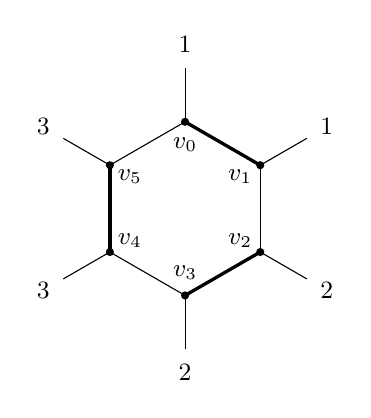
\begin{tikzpicture}[scale=1.05,every node/.style={font=\small}]
  \foreach \i in {0,...,5} {
    \coordinate (v\i) at ({90-60*\i}:1.05);
    \coordinate (x\i) at ({90-60*\i}:1.7);
    \fill (v\i) circle (1.4pt);
    \node at ({90-60*\i}:.77) {$v_{\i}$};
    \draw (v\i)--(x\i);
  }
  \foreach \i/\j in {0/1,2/3,4/5} {\draw[very thick] (v\i)--(v\j);}
  \foreach \i/\j in {1/2,3/4,5/0} {\draw (v\i)--(v\j);}
  \foreach \i/\c in {0/1,1/1,2/2,3/2,4/3,5/3} {
    \node at ({90-60*\i}:1.98) {$\c$};
  }
\end{tikzpicture}
\caption{The spoke colours. The thick hexagon edges join
equal-coloured spokes; the other three hexagon edges form $U$.}
\label{fig:hexagon}
\end{figure}
\FloatBarrier

\subsection{Three 2-factors}

The colouring $f$ gives three perfect matchings $M_1,M_2,M_3$.
For $i\in\{1,2,3\}$, take the edges outside $H$ of colour $i$, together
with each of $e_0,e_2,e_4$ whose incident spokes have a colour different
from $i$. Exactly one edge is selected at each hexagon vertex.
Hence each $M_i$ is a perfect matching.
Put
\[
  B_i=E(G)\setminus M_i,\qquad U=\{e_1,e_3,e_5\}.
\]
Each $B_i$ is even. Edges outside $H$ occur in two of the $B_i$;
edges $e_0,e_2,e_4$ occur in one; and edges in $U$ occur in all three.

\Needspace{9\baselineskip}
\begin{lemma}\label{lem:alternating}
If $F$ is even and $F\cap E(H)=U$, then
\begin{equation}\label{eq:alternating}
  F,\quad H,\quad F\sd B_1,\quad F\sd B_2,\quad F\sd B_3
\end{equation}
is a five-cycle double cover of $G$.
\end{lemma}

\begin{proof}
An edge outside $H$ belongs to two of the $B_i$. If it belongs to
$F$, it therefore belongs to exactly one of the three $F\sd B_i$,
and $F$ supplies its second occurrence. If it does not belong to
$F$, it belongs to two of the $F\sd B_i$. Each edge of $H\setminus U$ belongs
to one $B_i$ and to $H$, and does not belong to $F$. Each edge of
$U$ belongs to $F$ and $H$, and to none of the $F\sd B_i$.
All five members are even.
\end{proof}

In particular, an even set $F=C\cup D$ with $D$ vertex-disjoint from
$C$ makes $C$ a component of the first member of \eqref{eq:alternating}.
We next construct $D$ in the intersection case that requires it.

\subsection{A circuit meeting the hexagon}

Let $C$ be a circuit meeting $H$. At each common vertex, the two pairs
of edges used by $C$ and $H$ share an edge, by cubicity. Thus every
common vertex has a neighbour that is also common. There are either
at least three common vertices or exactly the ends of one shared edge.

Suppose first that $|V(C)\cap V(H)|\geq3$. The surviving part of $H$
in $G-V(C)$ consists of paths on at most three vertices. Retain $f$
outside $H$. A single edge can avoid both of its endpoint spoke
colours. On a three-vertex path, let its spoke colours be $a,b,c$.
For $a=b$, choose the edge at the opposite end first, avoiding $b,c$,
and give the other edge the remaining colour different from $a,b$.
The case $b=c$ is symmetric. For three distinct colours, give the
first edge colour $c$ and the second colour $a$. Every consecutive
triple in \eqref{eq:hexword} has one of these forms. A deleted spoke
allows the same colouring to be restricted to the surviving edges.
Thus $G-V(C)$ is 3-edge-colourable, and \cref{thm:exact} gives a
five-cycle double cover with $C$ as a member.

If the two common vertices are $v_j,v_{j+1}$ with $j$ even, deleting
them leaves a four-vertex path with spoke colours $2,2,3,3$, after
cyclic relabelling of the colours. Its three edges can be coloured
$3,1,2$. Again \cref{thm:exact} applies.

It remains to treat two common vertices at an edge of $U$. Rotate
the indices and permute the colours so that the shared edge is $e_0$
and the cyclic list of spoke colours becomes
\begin{equation}\label{eq:shiftedword}
  (1,2,2,3,3,1).
\end{equation}
In these coordinates, $U=\{e_0,e_2,e_4\}$ and the four surviving
spokes have outer endpoints $x_2,x_3,x_4,x_5$. Let
$R=G-V(C\cup H)$.

\Needspace{11\baselineskip}
\begin{lemma}\label{lem:fourterm}
In the coordinates of \eqref{eq:shiftedword}, one of the following
exists.
\begin{enumerate}
\item A proper 3-edge-colouring of $G-V(C)$.
\item An even subgraph $D$, vertex-disjoint from $C$, such that
$D\cap E(H)=\{e_2,e_4\}$.
\end{enumerate}
\end{lemma}

\begin{proof}
First suppose that all four $x_2,x_3,x_4,x_5$ lie outside $C$, and
that every component of $R$ contains an even number of these four
endpoints, counted with repetition. The edge set
\[
  Q=\{s_2,s_3,s_4,s_5,e_2,e_4\}
\]
has even degree at each hexagon vertex, and its boundary in $R$ is
the set of vertices occurring an odd number of times among
$x_2,x_3,x_4,x_5$. By \cref{lem:join}, an
edge set $J\subseteq E(R)$ has this same boundary. The union
$D=Q\cup J$ is even, avoids $C$, and has the asserted hexagon edges.

The other configurations admit a recolouring of the four-vertex
path. The following table changes just one of its spoke colours.
The last column gives the colours of $e_2,e_3,e_4$ in that order.
\begin{center}
\small
\begin{tabular}{@{}ccc@{}}
\toprule
Endpoint & New spoke colours at $v_2,v_3,v_4,v_5$ & Path colours\\
\midrule
$x_2$ & $1,3,3,1$ & $2,1,2$\\
$x_3$ & $2,2,3,1$ & $3,1,2$\\
$x_4$ & $2,3,1,1$ & $1,2,3$\\
$x_5$ & $2,3,3,2$ & $1,2,1$\\
\bottomrule
\end{tabular}
\end{center}
Each row gives three distinct colours at the two internal path
vertices and a path-edge colour different from the endpoint spoke
colour. If some $x_t$ lies on $C$, its spoke is deleted from $G-V(C)$.
Use the row for $x_t$ and retain $f$ on every surviving edge outside $H$.

Otherwise all four endpoints lie in $R$, and some component contains
an odd number of them, counted with repetition. That component, or
the union of the other components, contains exactly one of the four,
say the one at $x_t$. Apply throughout those components the
transposition of the original colour of $s_t$ and the new colour in
the corresponding table row. Apply the same transposition to all
edges from these components to $H$. Properness is preserved at every
vertex of $R$, and among the four surviving spokes exactly $s_t$
changes colour. The table now completes a proper colouring of
$G-V(C)$.
\end{proof}

In the first case of \cref{lem:fourterm}, \cref{thm:exact} gives a
five-cycle double cover with $C$ as a member. In the second, $C$ uses
exactly $e_0$ of the hexagon, so $F=C\cup D$ satisfies the hypothesis of
\cref{lem:alternating}. The resulting cover has $C$ as a component.
This settles every circuit meeting $H$.

\section{A circuit disjoint from the hexagon}\label{sec:disjoint}

Keep $G,H$ and $f$ as in \cref{sec:hexagon}. Let $C$ be a circuit of
$G$ vertex-disjoint from $H$, and put $R=G-V(C\cup H)$. We use two
elementary operations on covers before considering the possible
connections among the six spokes.

\Needspace{10\baselineskip}
\begin{lemma}\label{lem:toggle}
Let $K$ be a properly 3-edge-coloured cubic graph, and let $B_i$ be
the union of its two colour classes other than $i$. If $C,D$ are
vertex-disjoint even subgraphs, then
\begin{equation}\label{eq:toggle}
 C,\quad D,\quad B_1\sd C\sd D,\quad
 B_2\sd C\sd D,\quad B_3\sd C\sd D
\end{equation}
is a five-cycle double cover of $K$.
\end{lemma}

\begin{proof}
Every edge belongs to two of the $B_i$. An edge of $C\cup D$
therefore belongs to exactly one of the three $B_i\sd C\sd D$;
$C$ or $D$ supplies its second occurrence. Every other edge belongs
to two of these symmetric differences. All five members are even.
\end{proof}

Label an edge of a double cover by the pair of indices of the members
containing it. Evenness of each member means that every index occurs
an even number of times at each vertex.

\Needspace{18\baselineskip}
\begin{lemma}[Restoring the hexagon]\label{lem:restore}
Suppose that the edges outside $H$ are labelled by pairs of cover
indices, with each index occurring an even number of times at every
vertex outside $H$. Suppose that the six spoke labels, in order, are
\[
 \{s,a\},\{s,a\},\{s,b\},\{s,b\},\{s,c\},\{s,c\},
\]
where $s,a,b,c$ are distinct. Introduce a fresh index $h$, and label
the hexagon edges $e_0,\dots,e_5$ by
\begin{equation}\label{eq:restore}
 \{a,h\},\{s,h\},\{b,h\},\{s,h\},\{c,h\},\{s,h\}.
\end{equation}
These labels define a double cover of $G$, with $H$ itself as member $h$.
If $C$ is already a member, is disjoint from $H$, and has an index
different from $s,a,b,c$, then $C$ remains a member.
\end{lemma}

\begin{proof}
At each hexagon vertex the three incident pairs are the three sides
of a triangle on three indices. Every index therefore has degree
zero or two there. All edges receive exactly two indices, and $h$
occurs precisely on $H$.
\end{proof}

In the applications below, the initial cover has five members and
contains $C$ as a member. After \cref{lem:restore} adds $H$ as a
member, replace $C$ and $H$ by $C\cup H$. This gives a five-cycle
double cover with $C$ as a component of one member.

\subsection{Connecting an equal-coloured pair}

Suppose that some pair of spokes with the same colour has its outer
endpoints in the same component of $R$. By an even rotation and a
colour permutation, take this pair to be $s_0,s_1$, of colour 1.
Delete $H$, and replace the three equal-coloured spoke pairs by new
edges $x_0x_1,x_2x_3,x_4x_5$, coloured 1, 2, 3, respectively.
The resulting cubic multigraph $K$ is properly coloured by the
extended $f$. Each new edge has distinct ends, since equal-coloured
spokes have distinct outer endpoints in a proper colouring.

Choose a path in $R$ from $x_0$ to $x_1$. Together with the first
edge it forms a circuit $D$ of $K$ disjoint from $C$. Apply
\cref{lem:toggle}, with member indices $\mathsf c,\mathsf d,1,2,3$
for $C,D$ and the three symmetric differences. The first new edge has label
$\{\mathsf d,1\}$. The second and third new edges have labels
$\{1,3\}$ and $\{1,2\}$. Replace each new edge by its two original
spokes, giving both spokes that edge's label. Their ordered labels are
\[
 \{1,\mathsf d\},\{1,\mathsf d\},
 \{1,3\},\{1,3\},\{1,2\},\{1,2\}.
\]
Apply \cref{lem:restore} with $s=1$, $a=\mathsf d$, $b=3$, $c=2$.
Replace the members $C$ and $H$ by their union to obtain the
required five-cycle double cover.

\subsection{Permuting colours in the remaining components}

We may now assume that the two outer endpoints of each equal-coloured
pair belong to different components of $R$, or that at least one of
them lies on $C$. Partition the positions $0,\dots,5$ according to
the components of $R$ containing their outer endpoints. Give each
spoke directly joining $H$ to $C$ its own singleton block. No block
contains $\{0,1\}$, $\{2,3\}$ or $\{4,5\}$.

On each component of $R$, we may independently permute the three
colours, including on its incident spokes to $H$. The proper colouring
is preserved on $R$. A spoke to $C$ is deleted from $G-V(C)$, so its
colour in the local completion may be chosen freely.

\Needspace{11\baselineskip}
\begin{lemma}\label{lem:partition}
Let $\mathcal P$ be a partition of $\{0,\dots,5\}$ with each of
$\{0,1\}$, $\{2,3\}$ and $\{4,5\}$ split between blocks. Starting
from the spoke colours $1,1,2,2,3,3$, independent colour permutations
on the blocks give spoke colours that extend to a proper colouring of the
hexagon whenever
\[
 \mathcal P\ne\bigl\{\{0,3\},\{1,4\},\{2,5\}\bigr\}.
\]
\end{lemma}

\begin{proof}
Coarsen $\mathcal P$ until every pair of distinct blocks is joined
by one of the three original pairs $\{0,1\}$, $\{2,3\}$ and
$\{4,5\}$. Such a coarsening preserves the hypothesis. Regard the
original pairs as three edges on the set of blocks. The resulting
underlying graph is complete, so it has two blocks or three blocks
forming a triangle. The twelve possibilities are listed below.
In the first column, positions carrying the same digit belong to the
same block; digits are assigned in order of first occurrence.

\begin{center}
\small
\begin{tabular}{@{}ccc@{}}
\toprule
Partition & Spoke colours & Colours of $e_0,\dots,e_5$\\
\midrule
\word{010101} & \word{112332} & \word{231213}\\
\word{010110} & \word{122133} & \word{313212}\\
\word{010212} & \word{112332} & \word{231213}\\
\word{010221} & \word{122133} & \word{313212}\\
\word{011001} & \word{132231} & \word{213123}\\
\word{011010} & \word{113223} & \word{321312}\\
\word{011202} & \word{112332} & \word{231213}\\
\word{011220} & \word{123123} & \word{312312}\\
\word{012012} & \multicolumn{2}{c}{opposite-pair partition}\\
\word{012021} & \word{113223} & \word{321312}\\
\word{012102} & \word{122133} & \word{313212}\\
\word{012120} & \word{113223} & \word{321312}\\
\bottomrule
\end{tabular}
\end{center}
For each displayed colouring, equalities and inequalities of the
original spoke colours are preserved within every block. Thus each
block assignment extends to a permutation of the three colours.
At each hexagon vertex the spoke and its two incident hexagon edges
have the three distinct colours. The same assignment works for every
refinement of that block partition.

If $\mathcal P$ is a proper refinement of the opposite-pair
partition, some opposite pair is split. An even rotation places that
pair at $\{0,3\}$ and permutes the original three spoke colours.
The partition then also refines
$\{\{0,2,5\},\{1,3,4\}\}$, represented by \word{010110}.
Its row gives the required completion.
\end{proof}

Whenever \cref{lem:partition} applies, combine its local completion
with the permuted colourings of $R$, and restrict to $G-V(C)$.
This gives a proper 3-edge-colouring. By \cref{thm:exact}, the
circuit $C$ is a member of a five-cycle double cover.

\subsection{Three pairs of opposite vertices}

The remaining partition has three blocks
$\{0,3\}$, $\{1,4\}$ and $\{2,5\}$. All six spokes end in $R$,
and each opposite pair has its endpoints in its own component.
Replace $H$ by a claw with centre $z$ and leaves $w_0,w_1,w_2$.
Attach the spokes formerly at $v_i,v_{i+3}$ to $w_i$, for $i=0,1,2$.
Their colour pairs are $\{1,2\}$, $\{1,3\}$ and $\{2,3\}$.
Colour the central edges $zw_0,zw_1,zw_2$ with $3,2,1$,
respectively. This gives a properly coloured cubic multigraph $K$.

In each of the three components of $R$, choose a path between the
two endpoints of its opposite spokes. The path and the two spoke
edges at $w_i$ form a circuit $D_i$. Coincident endpoints give a
path of length zero and a two-edge circuit. The three circuits are
vertex-disjoint and avoid $C$. Set $D=D_0\cup D_1\cup D_2$ and
apply \cref{lem:toggle}, again with indices
$\mathsf c,\mathsf d,1,2,3$.

Every spoke edge belongs to $D$. A spoke of original colour $j$
therefore has cover label $\{\mathsf d,j\}$. Delete the claw and
restore the original six spokes. Their labels, in hexagon order, are
\[
 \{\mathsf d,1\},\{\mathsf d,1\},
 \{\mathsf d,2\},\{\mathsf d,2\},
 \{\mathsf d,3\},\{\mathsf d,3\}.
\]
Use \cref{lem:restore} with $s=\mathsf d$, $a=1$, $b=2$, $c=3$.
Replace the members $C$ and $H$ by their union to obtain a five-cycle
double cover with $C$ as a component. Every circuit
disjoint from $H$ has now been treated.

\newpage
\section{Strong covers}\label{sec:conclusion}

\Needspace{11\baselineskip}
\inducedhexagon*
\begin{proof}
Let $G$ and $H$ satisfy the hypotheses, and let $C$ be an arbitrary
circuit of $G$. If $C$ meets $H$, the constructions in
\cref{sec:hexagon} give either a five-cycle double cover with $C$
as a member or the
cover of \cref{lem:alternating} with $C\cup D$ as one member,
where $D$ is vertex-disjoint from $C$. If $C$ is vertex-disjoint from $H$,
\cref{sec:disjoint} gives a five-cycle double cover with $C$ as a
member or a cover
having $C\cup H$ as one member. Thus every circuit is a component
of a member of a five-cycle double cover.

\end{proof}

\Needspace{8\baselineskip}
\defectthree*
\begin{proof}
Let $G$ be a snark with $\df(G)=3$. By \citep{KMNS24}, Theorem~3.3,
$G$ has an induced hexagon $H$ with a proper 3-edge-colouring of
$G-E(H)$ whose
spoke colours are $1,1,2,2,3,3$, after a rotation and colour permutation.
Apply \cref{thm:hexagon}.
\end{proof}

For an individual circuit $C$ in a snark of colouring defect three,
\cref{thm:exact} also decides whether $C$ itself can be a member of
a five-cycle double cover: this holds if and only if $G-V(C)$ is
3-edge-colourable.

\newpage
tt

For context, we recall how the classes considered here relate to two
further familiar classes. A snark $G$ is \emph{hypohamiltonian} if
$G-v$ has a Hamiltonian circuit for every vertex $v$ (while $G$
itself has none). It is \emph{bicritical} if $G-\{u,v\}$ is
3-edge-colourable for every pair of distinct vertices $u,v$, rather
than only for adjacent pairs as in the definition of criticality.

Every hypohamiltonian snark is bicritical, and every bicritical snark
is critical. Both inclusions are strict. Steffen \bothcite{S01},
Theorem~2.4 and the following remark, records the first inclusion and
the bicritical, non-hypohamiltonian Goldberg snarks on 22 vertices.
Critical snarks that are not bicritical are discussed by
M\'a\v{c}ajov\'a and \v{S}koviera \bothcite{MS21}, Section~3;
such examples occur at every even order at least 32. Bicritical
snarks are also precisely the irreducible snarks
\citep[Theorem~6]{MS21}.

Permutation snarks are conjecturally bicritical. Equivalently, the
conjecture asks whether every permutation snark is critical.
M\'a\v{c}ajov\'a and \v{S}koviera \bothcite{MS25} study the
criticality question and report that all permutation snarks with
fewer than 50 vertices are bicritical. Their Theorem~1.1 shows that
a noncritical permutation snark would imply the existence of a
permutation snark of order $6\pmod 8$.

The equivalence concerns the two assertions about the whole class.
Indeed, in a permutation snark a pair whose deletion leaves an
uncolourable graph must lie on the same defining circuit: deleting
one vertex from each circuit leaves two paths, which can be coloured
alternately with two colours, with the matching coloured by the third.
If the pair on one circuit is nonadjacent, reconnect that circuit to
make the pair adjacent, changing only one other edge outside the pair.
The resulting graph is still a permutation graph, and deleting the
pair leaves a graph containing the original uncolourable remainder.
Thus a counterexample to the bicritical formulation yields a
counterexample to the critical formulation.

\Needspace{12\baselineskip}
\begin{figure}[htbp]
\centering
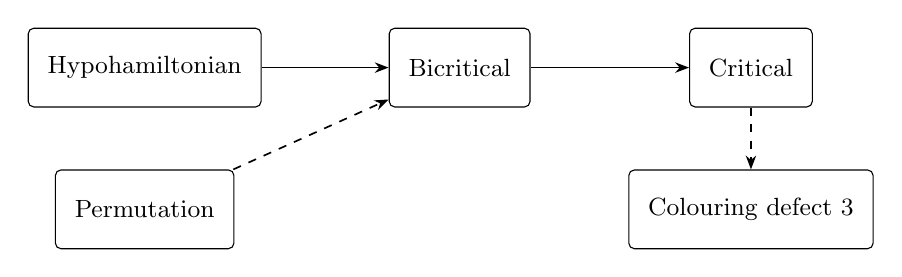
\begin{tikzpicture}[
  every node/.style={font=\small},
  class/.style={draw,rounded corners=2pt,align=center,
    minimum height=10mm,inner xsep=7pt},
  inclusion/.style={-{Stealth[length=5pt]},line width=.6pt},
  conjecture/.style={inclusion,dashed}]
  \node[class] (hypo) at (0,0) {Hypohamiltonian};
  \node[class] (bicrit) at (4,0) {Bicritical};
  \node[class] (crit) at (7.7,0) {Critical};
  \node[class] (perm) at (0,-1.8) {Permutation};
  \node[class] (defect) at (7.7,-1.8) {Colouring defect 3};
  \draw[inclusion] (hypo) -- (bicrit);
  \draw[inclusion] (bicrit) -- (crit);
  \draw[conjecture] (perm) -- (bicrit);
  \draw[conjecture] (crit) -- (defect);
\end{tikzpicture}
\caption{Relationships between classes of snarks. Solid arrows are
proved inclusions, both strict; dashed arrows are conjectural
inclusions. The dashed arrow from permutation to bicritical can
equivalently be directed to critical. The conjecture that critical
snarks have defect 3 implies the corresponding conjectures for
bicritical and hypohamiltonian snarks.}
\label{fig:snark-classes}
\end{figure}
\FloatBarrier

Karab\'a\v{s}, M\'a\v{c}ajov\'a, Nedela and \v{S}koviera
\citep[Conjecture~7.4]{KMNS24} conjecture that every critical snark
has colouring defect three. Their Conjecture~7.6 makes the weaker
assertion for irreducible, equivalently bicritical, snarks. Both imply
Steffen's earlier conjecture \bothcite{S15}, Conjecture~4.1, that
every hypohamiltonian snark has defect three (his $\mu_3$ is our
$\df$). Together with the permutation criticality conjecture, they
would also put every permutation snark in the defect-three class.
Defect three does not imply criticality, even for cyclically
4-edge-connected snarks of girth at least five: the six snarks on
20 vertices in \citep[Table~1]{KMNS24} all have defect three, but
only one is critical.

\newpage
\begingroup
\fontsize{10}{12}\selectfont
\setlength{\bibsep}{5pt}
\begin{thebibliography}{KMNS24}
\bibitem[HO13]{HO13}\paperreference{HO13}
\bibitem[HOZZ19]{HOZZ19}\paperreference{HOZZ19}
\bibitem[HS26]{HS26}\paperreference{HS26}
\bibitem[KMNS24]{KMNS24}\paperreference{KMNS24}
\bibitem[LHLZ25]{LHLZ25}\paperreference{LHLZ25}
\bibitem[LHLZ23]{LHLZ23}\paperreference{LHLZ23}
\bibitem[MS21]{MS21}\paperreference{MS21}
\bibitem[MS25]{MS25}\paperreference{MS25}
\bibitem[S01]{S01}\paperreference{S01}
\bibitem[S15]{S15}\paperreference{S15}
\bibitem[U26]{U26}\paperreference{U26}
\bibitem[Xu14]{Xu14}\paperreference{Xu14}
\end{thebibliography}
\endgroup
\end{document}
